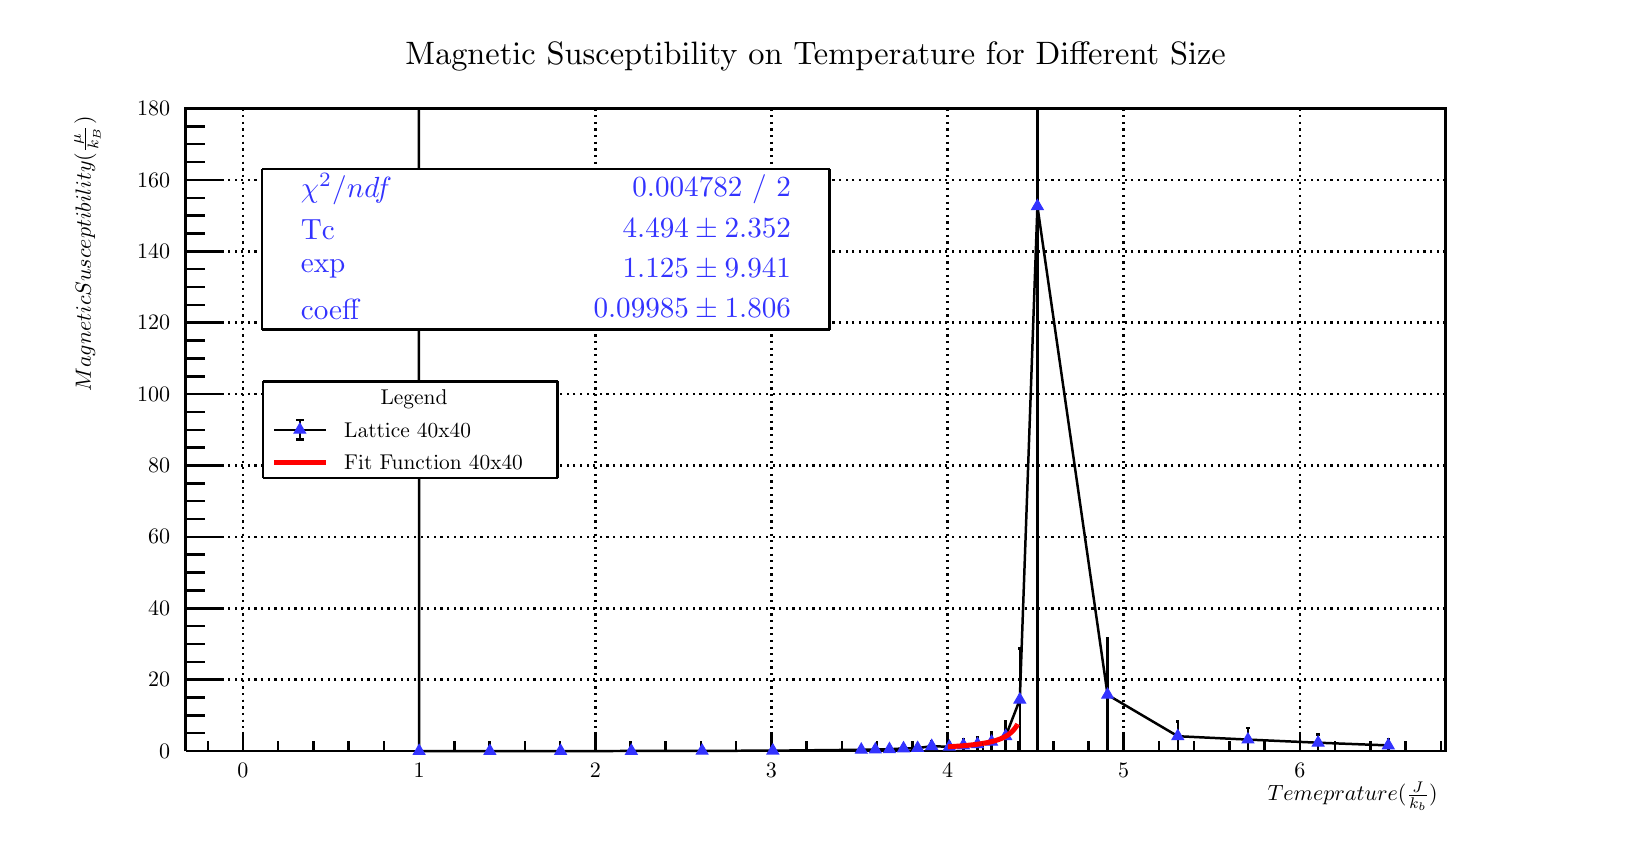
\begin{tikzpicture}
\pgfdeclareplotmark{cross} {
\pgfpathmoveto{\pgfpoint{-0.3\pgfplotmarksize}{\pgfplotmarksize}}
\pgfpathlineto{\pgfpoint{+0.3\pgfplotmarksize}{\pgfplotmarksize}}
\pgfpathlineto{\pgfpoint{+0.3\pgfplotmarksize}{0.3\pgfplotmarksize}}
\pgfpathlineto{\pgfpoint{+1\pgfplotmarksize}{0.3\pgfplotmarksize}}
\pgfpathlineto{\pgfpoint{+1\pgfplotmarksize}{-0.3\pgfplotmarksize}}
\pgfpathlineto{\pgfpoint{+0.3\pgfplotmarksize}{-0.3\pgfplotmarksize}}
\pgfpathlineto{\pgfpoint{+0.3\pgfplotmarksize}{-1.\pgfplotmarksize}}
\pgfpathlineto{\pgfpoint{-0.3\pgfplotmarksize}{-1.\pgfplotmarksize}}
\pgfpathlineto{\pgfpoint{-0.3\pgfplotmarksize}{-0.3\pgfplotmarksize}}
\pgfpathlineto{\pgfpoint{-1.\pgfplotmarksize}{-0.3\pgfplotmarksize}}
\pgfpathlineto{\pgfpoint{-1.\pgfplotmarksize}{0.3\pgfplotmarksize}}
\pgfpathlineto{\pgfpoint{-0.3\pgfplotmarksize}{0.3\pgfplotmarksize}}
\pgfpathclose
\pgfusepathqstroke
}
\pgfdeclareplotmark{cross*} {
\pgfpathmoveto{\pgfpoint{-0.3\pgfplotmarksize}{\pgfplotmarksize}}
\pgfpathlineto{\pgfpoint{+0.3\pgfplotmarksize}{\pgfplotmarksize}}
\pgfpathlineto{\pgfpoint{+0.3\pgfplotmarksize}{0.3\pgfplotmarksize}}
\pgfpathlineto{\pgfpoint{+1\pgfplotmarksize}{0.3\pgfplotmarksize}}
\pgfpathlineto{\pgfpoint{+1\pgfplotmarksize}{-0.3\pgfplotmarksize}}
\pgfpathlineto{\pgfpoint{+0.3\pgfplotmarksize}{-0.3\pgfplotmarksize}}
\pgfpathlineto{\pgfpoint{+0.3\pgfplotmarksize}{-1.\pgfplotmarksize}}
\pgfpathlineto{\pgfpoint{-0.3\pgfplotmarksize}{-1.\pgfplotmarksize}}
\pgfpathlineto{\pgfpoint{-0.3\pgfplotmarksize}{-0.3\pgfplotmarksize}}
\pgfpathlineto{\pgfpoint{-1.\pgfplotmarksize}{-0.3\pgfplotmarksize}}
\pgfpathlineto{\pgfpoint{-1.\pgfplotmarksize}{0.3\pgfplotmarksize}}
\pgfpathlineto{\pgfpoint{-0.3\pgfplotmarksize}{0.3\pgfplotmarksize}}
\pgfpathclose
\pgfusepathqfillstroke
}
\pgfdeclareplotmark{newstar} {
\pgfpathmoveto{\pgfqpoint{0pt}{\pgfplotmarksize}}
\pgfpathlineto{\pgfqpointpolar{44}{0.5\pgfplotmarksize}}
\pgfpathlineto{\pgfqpointpolar{18}{\pgfplotmarksize}}
\pgfpathlineto{\pgfqpointpolar{-20}{0.5\pgfplotmarksize}}
\pgfpathlineto{\pgfqpointpolar{-54}{\pgfplotmarksize}}
\pgfpathlineto{\pgfqpointpolar{-90}{0.5\pgfplotmarksize}}
\pgfpathlineto{\pgfqpointpolar{234}{\pgfplotmarksize}}
\pgfpathlineto{\pgfqpointpolar{198}{0.5\pgfplotmarksize}}
\pgfpathlineto{\pgfqpointpolar{162}{\pgfplotmarksize}}
\pgfpathlineto{\pgfqpointpolar{134}{0.5\pgfplotmarksize}}
\pgfpathclose
\pgfusepathqstroke
}
\pgfdeclareplotmark{newstar*} {
\pgfpathmoveto{\pgfqpoint{0pt}{\pgfplotmarksize}}
\pgfpathlineto{\pgfqpointpolar{44}{0.5\pgfplotmarksize}}
\pgfpathlineto{\pgfqpointpolar{18}{\pgfplotmarksize}}
\pgfpathlineto{\pgfqpointpolar{-20}{0.5\pgfplotmarksize}}
\pgfpathlineto{\pgfqpointpolar{-54}{\pgfplotmarksize}}
\pgfpathlineto{\pgfqpointpolar{-90}{0.5\pgfplotmarksize}}
\pgfpathlineto{\pgfqpointpolar{234}{\pgfplotmarksize}}
\pgfpathlineto{\pgfqpointpolar{198}{0.5\pgfplotmarksize}}
\pgfpathlineto{\pgfqpointpolar{162}{\pgfplotmarksize}}
\pgfpathlineto{\pgfqpointpolar{134}{0.5\pgfplotmarksize}}
\pgfpathclose
\pgfusepathqfillstroke
}
\definecolor{c}{rgb}{1,1,1};
\draw [color=c, fill=c] (0,0) rectangle (20,10.2002);
\draw [color=c, fill=c] (2,1.02002) rectangle (18,9.18019);
\definecolor{c}{rgb}{0,0,0};
\draw [c,line width=0.9] (2,1.02002) -- (2,9.18019) -- (18,9.18019) -- (18,1.02002) -- (2,1.02002);
\definecolor{c}{rgb}{1,1,1};
\draw [color=c, fill=c] (2,1.02002) rectangle (18,9.18019);
\definecolor{c}{rgb}{0,0,0};
\draw [c,line width=0.9] (2,1.02002) -- (2,9.18019) -- (18,9.18019) -- (18,1.02002) -- (2,1.02002);
\draw [c,line width=0.9] (2,1.02002) -- (18,1.02002);
\draw [c,dash pattern=on 0.80pt off 1.60pt ,line width=0.9] (2.72726,9.18019) -- (2.72726,1.02002);
\draw [c,dash pattern=on 0.80pt off 1.60pt ,line width=0.9] (4.96433,9.18019) -- (4.96433,1.02002);
\draw [c,dash pattern=on 0.80pt off 1.60pt ,line width=0.9] (7.2014,9.18019) -- (7.2014,1.02002);
\draw [c,dash pattern=on 0.80pt off 1.60pt ,line width=0.9] (9.43847,9.18019) -- (9.43847,1.02002);
\draw [c,dash pattern=on 0.80pt off 1.60pt ,line width=0.9] (11.6755,9.18019) -- (11.6755,1.02002);
\draw [c,dash pattern=on 0.80pt off 1.60pt ,line width=0.9] (13.9126,9.18019) -- (13.9126,1.02002);
\draw [c,dash pattern=on 0.80pt off 1.60pt ,line width=0.9] (16.1497,9.18019) -- (16.1497,1.02002);
\draw [c,dash pattern=on 0.80pt off 1.60pt ,line width=0.9] (2.72726,9.18019) -- (2.72726,1.02002);
\draw [c,dash pattern=on 0.80pt off 1.60pt ,line width=0.9] (16.1497,9.18019) -- (16.1497,1.02002);
\draw [c,line width=0.9] (2,1.02002) -- (2,9.18019);
\draw [c,dash pattern=on 0.80pt off 1.60pt ,line width=0.9] (18,1.02002) -- (2,1.02002);
\draw [c,dash pattern=on 0.80pt off 1.60pt ,line width=0.9] (18,1.92671) -- (2,1.92671);
\draw [c,dash pattern=on 0.80pt off 1.60pt ,line width=0.9] (18,2.83339) -- (2,2.83339);
\draw [c,dash pattern=on 0.80pt off 1.60pt ,line width=0.9] (18,3.74008) -- (2,3.74008);
\draw [c,dash pattern=on 0.80pt off 1.60pt ,line width=0.9] (18,4.64676) -- (2,4.64676);
\draw [c,dash pattern=on 0.80pt off 1.60pt ,line width=0.9] (18,5.55345) -- (2,5.55345);
\draw [c,dash pattern=on 0.80pt off 1.60pt ,line width=0.9] (18,6.46013) -- (2,6.46013);
\draw [c,dash pattern=on 0.80pt off 1.60pt ,line width=0.9] (18,7.36682) -- (2,7.36682);
\draw [c,dash pattern=on 0.80pt off 1.60pt ,line width=0.9] (18,8.2735) -- (2,8.2735);
\draw [c,dash pattern=on 0.80pt off 1.60pt ,line width=0.9] (18,9.18019) -- (2,9.18019);
\draw [c,line width=0.9] (2,1.02002) -- (18,1.02002);
\draw [c,line width=0.9] (2.72726,1.26483) -- (2.72726,1.02002);
\draw [c,line width=0.9] (3.17468,1.14242) -- (3.17468,1.02002);
\draw [c,line width=0.9] (3.62209,1.14242) -- (3.62209,1.02002);
\draw [c,line width=0.9] (4.0695,1.14242) -- (4.0695,1.02002);
\draw [c,line width=0.9] (4.51692,1.14242) -- (4.51692,1.02002);
\draw [c,line width=0.9] (4.96433,1.26483) -- (4.96433,1.02002);
\draw [c,line width=0.9] (5.41174,1.14242) -- (5.41174,1.02002);
\draw [c,line width=0.9] (5.85916,1.14242) -- (5.85916,1.02002);
\draw [c,line width=0.9] (6.30657,1.14242) -- (6.30657,1.02002);
\draw [c,line width=0.9] (6.75399,1.14242) -- (6.75399,1.02002);
\draw [c,line width=0.9] (7.2014,1.26483) -- (7.2014,1.02002);
\draw [c,line width=0.9] (7.64881,1.14242) -- (7.64881,1.02002);
\draw [c,line width=0.9] (8.09623,1.14242) -- (8.09623,1.02002);
\draw [c,line width=0.9] (8.54364,1.14242) -- (8.54364,1.02002);
\draw [c,line width=0.9] (8.99105,1.14242) -- (8.99105,1.02002);
\draw [c,line width=0.9] (9.43847,1.26483) -- (9.43847,1.02002);
\draw [c,line width=0.9] (9.88588,1.14242) -- (9.88588,1.02002);
\draw [c,line width=0.9] (10.3333,1.14242) -- (10.3333,1.02002);
\draw [c,line width=0.9] (10.7807,1.14242) -- (10.7807,1.02002);
\draw [c,line width=0.9] (11.2281,1.14242) -- (11.2281,1.02002);
\draw [c,line width=0.9] (11.6755,1.26483) -- (11.6755,1.02002);
\draw [c,line width=0.9] (12.123,1.14242) -- (12.123,1.02002);
\draw [c,line width=0.9] (12.5704,1.14242) -- (12.5704,1.02002);
\draw [c,line width=0.9] (13.0178,1.14242) -- (13.0178,1.02002);
\draw [c,line width=0.9] (13.4652,1.14242) -- (13.4652,1.02002);
\draw [c,line width=0.9] (13.9126,1.26483) -- (13.9126,1.02002);
\draw [c,line width=0.9] (14.36,1.14242) -- (14.36,1.02002);
\draw [c,line width=0.9] (14.8074,1.14242) -- (14.8074,1.02002);
\draw [c,line width=0.9] (15.2548,1.14242) -- (15.2548,1.02002);
\draw [c,line width=0.9] (15.7023,1.14242) -- (15.7023,1.02002);
\draw [c,line width=0.9] (16.1497,1.26483) -- (16.1497,1.02002);
\draw [c,line width=0.9] (2.72726,1.26483) -- (2.72726,1.02002);
\draw [c,line width=0.9] (2.27985,1.14242) -- (2.27985,1.02002);
\draw [c,line width=0.9] (16.1497,1.26483) -- (16.1497,1.02002);
\draw [c,line width=0.9] (16.5971,1.14242) -- (16.5971,1.02002);
\draw [c,line width=0.9] (17.0445,1.14242) -- (17.0445,1.02002);
\draw [c,line width=0.9] (17.4919,1.14242) -- (17.4919,1.02002);
\draw [c,line width=0.9] (17.9393,1.14242) -- (17.9393,1.02002);
\draw [anchor=base] (2.72726,0.683414) node[scale=0.795711, color=c, rotate=0]{0};
\draw [anchor=base] (4.96433,0.683414) node[scale=0.795711, color=c, rotate=0]{1};
\draw [anchor=base] (7.2014,0.683414) node[scale=0.795711, color=c, rotate=0]{2};
\draw [anchor=base] (9.43847,0.683414) node[scale=0.795711, color=c, rotate=0]{3};
\draw [anchor=base] (11.6755,0.683414) node[scale=0.795711, color=c, rotate=0]{4};
\draw [anchor=base] (13.9126,0.683414) node[scale=0.795711, color=c, rotate=0]{5};
\draw [anchor=base] (16.1497,0.683414) node[scale=0.795711, color=c, rotate=0]{6};
\draw [anchor= east] (18,0.448809) node[scale=0.795711, color=c, rotate=0]{$Temeprature (\frac{J}{k_{b}})$};
\draw [c,line width=0.9] (2,1.02002) -- (2,9.18019);
\draw [c,line width=0.9] (2.48,1.02002) -- (2,1.02002);
\draw [c,line width=0.9] (2.24,1.24669) -- (2,1.24669);
\draw [c,line width=0.9] (2.24,1.47336) -- (2,1.47336);
\draw [c,line width=0.9] (2.24,1.70004) -- (2,1.70004);
\draw [c,line width=0.9] (2.48,1.92671) -- (2,1.92671);
\draw [c,line width=0.9] (2.24,2.15338) -- (2,2.15338);
\draw [c,line width=0.9] (2.24,2.38005) -- (2,2.38005);
\draw [c,line width=0.9] (2.24,2.60672) -- (2,2.60672);
\draw [c,line width=0.9] (2.48,2.83339) -- (2,2.83339);
\draw [c,line width=0.9] (2.24,3.06006) -- (2,3.06006);
\draw [c,line width=0.9] (2.24,3.28673) -- (2,3.28673);
\draw [c,line width=0.9] (2.24,3.51341) -- (2,3.51341);
\draw [c,line width=0.9] (2.48,3.74008) -- (2,3.74008);
\draw [c,line width=0.9] (2.24,3.96675) -- (2,3.96675);
\draw [c,line width=0.9] (2.24,4.19342) -- (2,4.19342);
\draw [c,line width=0.9] (2.24,4.42009) -- (2,4.42009);
\draw [c,line width=0.9] (2.48,4.64676) -- (2,4.64676);
\draw [c,line width=0.9] (2.24,4.87343) -- (2,4.87343);
\draw [c,line width=0.9] (2.24,5.10011) -- (2,5.10011);
\draw [c,line width=0.9] (2.24,5.32678) -- (2,5.32678);
\draw [c,line width=0.9] (2.48,5.55345) -- (2,5.55345);
\draw [c,line width=0.9] (2.24,5.78012) -- (2,5.78012);
\draw [c,line width=0.9] (2.24,6.00679) -- (2,6.00679);
\draw [c,line width=0.9] (2.24,6.23346) -- (2,6.23346);
\draw [c,line width=0.9] (2.48,6.46013) -- (2,6.46013);
\draw [c,line width=0.9] (2.24,6.6868) -- (2,6.6868);
\draw [c,line width=0.9] (2.24,6.91348) -- (2,6.91348);
\draw [c,line width=0.9] (2.24,7.14015) -- (2,7.14015);
\draw [c,line width=0.9] (2.48,7.36682) -- (2,7.36682);
\draw [c,line width=0.9] (2.24,7.59349) -- (2,7.59349);
\draw [c,line width=0.9] (2.24,7.82016) -- (2,7.82016);
\draw [c,line width=0.9] (2.24,8.04683) -- (2,8.04683);
\draw [c,line width=0.9] (2.48,8.2735) -- (2,8.2735);
\draw [c,line width=0.9] (2.24,8.50018) -- (2,8.50018);
\draw [c,line width=0.9] (2.24,8.72685) -- (2,8.72685);
\draw [c,line width=0.9] (2.24,8.95352) -- (2,8.95352);
\draw [c,line width=0.9] (2.48,9.18019) -- (2,9.18019);
\draw [anchor= east] (1.9,1.02002) node[scale=0.795711, color=c, rotate=0]{0};
\draw [anchor= east] (1.9,1.92671) node[scale=0.795711, color=c, rotate=0]{20};
\draw [anchor= east] (1.9,2.83339) node[scale=0.795711, color=c, rotate=0]{40};
\draw [anchor= east] (1.9,3.74008) node[scale=0.795711, color=c, rotate=0]{60};
\draw [anchor= east] (1.9,4.64676) node[scale=0.795711, color=c, rotate=0]{80};
\draw [anchor= east] (1.9,5.55345) node[scale=0.795711, color=c, rotate=0]{100};
\draw [anchor= east] (1.9,6.46013) node[scale=0.795711, color=c, rotate=0]{120};
\draw [anchor= east] (1.9,7.36682) node[scale=0.795711, color=c, rotate=0]{140};
\draw [anchor= east] (1.9,8.2735) node[scale=0.795711, color=c, rotate=0]{160};
\draw [anchor= east] (1.9,9.18019) node[scale=0.795711, color=c, rotate=0]{180};
\draw [anchor= east] (0.752055,9.18019) node[scale=0.795711, color=c, rotate=90]{$Magnetic Susceptibility (\frac{\mu}{k_{B}})$};
\draw [c,line width=0.9] (11.4744,1.12454) -- (11.4744,1.14476);
\draw [c,line width=0.9] (11.4533,1.14476) -- (11.4954,1.14476);
\draw [c,line width=0.9] (11.4744,1.04024) -- (11.4744,1.02002);
\draw [c,line width=0.9] (11.4533,1.02002) -- (11.4954,1.02002);
\draw [c,line width=0.9] (11.6981,1.11618) -- (11.6981,1.12804);
\draw [c,line width=0.9] (11.677,1.12804) -- (11.7192,1.12804);
\draw [c,line width=0.9] (11.6981,1.03188) -- (11.6981,1.02002);
\draw [c,line width=0.9] (11.677,1.02002) -- (11.7192,1.02002);
\draw [c,line width=0.9] (11.877,1.13433) -- (11.877,1.16434);
\draw [c,line width=0.9] (11.856,1.16434) -- (11.8981,1.16434);
\draw [c,line width=0.9] (11.877,1.05003) -- (11.877,1.02002);
\draw [c,line width=0.9] (11.856,1.02002) -- (11.8981,1.02002);
\draw [c,line width=0.9] (12.056,1.1486) -- (12.056,1.19288);
\draw [c,line width=0.9] (12.0349,1.19288) -- (12.0771,1.19288);
\draw [c,line width=0.9] (12.056,1.0643) -- (12.056,1.02002);
\draw [c,line width=0.9] (12.0349,1.02002) -- (12.0771,1.02002);
\draw [c,line width=0.9] (12.235,1.17941) -- (12.235,1.25451);
\draw [c,line width=0.9] (12.2139,1.25451) -- (12.256,1.25451);
\draw [c,line width=0.9] (12.235,1.09511) -- (12.235,1.02002);
\draw [c,line width=0.9] (12.2139,1.02002) -- (12.256,1.02002);
\draw [c,line width=0.9] (12.4139,1.25179) -- (12.4139,1.39925);
\draw [c,line width=0.9] (12.3929,1.39925) -- (12.435,1.39925);
\draw [c,line width=0.9] (12.4139,1.16749) -- (12.4139,1.02002);
\draw [c,line width=0.9] (12.3929,1.02002) -- (12.435,1.02002);
\draw [c,line width=0.9] (12.5929,1.71428) -- (12.5929,2.32424);
\draw [c,line width=0.9] (12.5718,2.32424) -- (12.614,2.32424);
\draw [c,line width=0.9] (12.5929,1.62998) -- (12.5929,1.02002);
\draw [c,line width=0.9] (12.5718,1.02002) -- (12.614,1.02002);
\draw [c,line width=0.9] (12.8166,7.98189) -- (12.8166,9.18019);
\draw [c,line width=0.9] (12.7955,9.18019) -- (12.8377,9.18019);
\draw [c,line width=0.9] (12.8166,7.89759) -- (12.8166,1.02002);
\draw [c,line width=0.9] (12.7955,1.02002) -- (12.8377,1.02002);
\draw [c,line width=0.9] (13.7078,1.77622) -- (13.7078,2.44812);
\draw [c,line width=0.9] (13.6868,2.44812) -- (13.7289,2.44812);
\draw [c,line width=0.9] (13.7078,1.69192) -- (13.7078,1.02002);
\draw [c,line width=0.9] (13.6868,1.02002) -- (13.7289,1.02002);
\draw [c,line width=0.9] (14.5991,1.25091) -- (14.5991,1.39751);
\draw [c,line width=0.9] (14.578,1.39751) -- (14.6201,1.39751);
\draw [c,line width=0.9] (14.5991,1.16661) -- (14.5991,1.02002);
\draw [c,line width=0.9] (14.578,1.02002) -- (14.6201,1.02002);
\draw [c,line width=0.9] (15.4903,1.20809) -- (15.4903,1.31187);
\draw [c,line width=0.9] (15.4692,1.31187) -- (15.5114,1.31187);
\draw [c,line width=0.9] (15.4903,1.12379) -- (15.4903,1.02002);
\draw [c,line width=0.9] (15.4692,1.02002) -- (15.5114,1.02002);
\draw [c,line width=0.9] (16.3815,1.16842) -- (16.3815,1.23252);
\draw [c,line width=0.9] (16.3604,1.23252) -- (16.4026,1.23252);
\draw [c,line width=0.9] (16.3815,1.08412) -- (16.3815,1.02002);
\draw [c,line width=0.9] (16.3604,1.02002) -- (16.4026,1.02002);
\draw [c,line width=0.9] (17.2727,1.13429) -- (17.2727,1.16427);
\draw [c,line width=0.9] (17.2517,1.16427) -- (17.2938,1.16427);
\draw [c,line width=0.9] (17.2727,1.05) -- (17.2727,1.02002);
\draw [c,line width=0.9] (17.2517,1.02002) -- (17.2938,1.02002);
\definecolor{c}{rgb}{1,1,1};
\draw [color=c, fill=c] (2.97155,6.37234) rectangle (10.1791,8.41462);
\definecolor{c}{rgb}{0,0,0};
\draw [c,line width=0.9] (2.97155,6.37234) -- (10.1791,6.37234);
\draw [c,line width=0.9] (10.1791,6.37234) -- (10.1791,8.41462);
\draw [c,line width=0.9] (10.1791,8.41462) -- (2.97155,8.41462);
\draw [c,line width=0.9] (2.97155,8.41462) -- (2.97155,6.37234);
\definecolor{c}{rgb}{0.2,0.2,1};
\draw [anchor= west] (3.33193,8.15933) node[scale=1.05315, color=c, rotate=0]{$\chi^{2} / ndf $};
\draw [anchor= east] (9.81876,8.15933) node[scale=1.05315, color=c, rotate=0]{ 0.004782 / 2};
\draw [anchor= west] (3.33193,7.64876) node[scale=1.05315, color=c, rotate=0]{Tc       };
\draw [anchor= east] (9.81876,7.64876) node[scale=1.05315, color=c, rotate=0]{$ 4.494 \pm 2.352$};
\draw [anchor= west] (3.33193,7.13819) node[scale=1.05315, color=c, rotate=0]{exp      };
\draw [anchor= east] (9.81876,7.13819) node[scale=1.05315, color=c, rotate=0]{$ 1.125 \pm 9.941$};
\draw [anchor= west] (3.33193,6.62763) node[scale=1.05315, color=c, rotate=0]{coeff    };
\draw [anchor= east] (9.81876,6.62763) node[scale=1.05315, color=c, rotate=0]{$ 0.09985 \pm 1.806$};
\definecolor{c}{rgb}{0,0,0};
\draw [c,line width=0.9] (4.9614,9.18019) -- (4.96434,1.02002);
\draw [c,line width=0.9] (4.96434,1.02002) -- (5.86277,1.02002) -- (6.76121,1.02002) -- (7.65964,1.02121) -- (8.55807,1.02289) -- (9.4565,1.02525) -- (10.5795,1.03654) -- (10.7585,1.03887) -- (10.9375,1.04325) -- (11.1164,1.05355) --
 (11.2954,1.05797) -- (11.4744,1.08239) -- (11.6981,1.07403) -- (11.877,1.09218) -- (12.056,1.10645) -- (12.235,1.13726) -- (12.4139,1.20964) -- (12.5929,1.67213) -- (12.8166,7.93974) -- (13.7078,1.73407) -- (14.5991,1.20876) -- (15.4903,1.16594) --
 (16.3815,1.12627) -- (17.2727,1.09215);
\definecolor{c}{rgb}{0.2,0.2,1};
\foreach \P in {(4.96434,1.02002), (5.86277,1.02009), (6.76121,1.02038), (7.65964,1.02121), (8.55807,1.02289), (9.4565,1.02525), (10.5795,1.03654), (10.7585,1.03887), (10.9375,1.04325), (11.1164,1.05355), (11.2954,1.05797), (11.4744,1.08239),
 (11.6981,1.07403), (11.877,1.09218), (12.056,1.10645), (12.235,1.13726), (12.4139,1.20964), (12.5929,1.67213), (12.8166,7.93974), (13.7078,1.73407), (14.5991,1.20876), (15.4903,1.16594), (16.3815,1.12627), (17.2727,1.09215)}{\draw[mark
 options={color=c,fill=c},mark size=2.402402pt,mark=triangle*] plot coordinates {\P};}
\definecolor{c}{rgb}{1,0,0};
\draw [c,line width=1.8] (11.68,1.07453) -- (11.689,1.07503) -- (11.6979,1.07555) -- (11.7069,1.07607) -- (11.7158,1.0766) -- (11.7248,1.07714) -- (11.7337,1.07769) -- (11.7427,1.07825) -- (11.7516,1.07882) -- (11.7605,1.0794) -- (11.7695,1.07999) --
 (11.7784,1.08059) -- (11.7874,1.08121) -- (11.7963,1.08183) -- (11.8053,1.08247) -- (11.8142,1.08312) -- (11.8232,1.08379) -- (11.8321,1.08446) -- (11.8411,1.08515) -- (11.85,1.08586) -- (11.859,1.08658) -- (11.8679,1.08731) -- (11.8769,1.08806) --
 (11.8858,1.08883) -- (11.8948,1.08961) -- (11.9037,1.09041) -- (11.9127,1.09123) -- (11.9216,1.09206) -- (11.9306,1.09292) -- (11.9395,1.09379) -- (11.9485,1.09468) -- (11.9574,1.0956) -- (11.9664,1.09653) -- (11.9753,1.09749) -- (11.9843,1.09847)
 -- (11.9932,1.09947) -- (12.0021,1.1005) -- (12.0111,1.10156) -- (12.02,1.10264) -- (12.029,1.10374) -- (12.0379,1.10488) -- (12.0469,1.10605) -- (12.0558,1.10724) -- (12.0648,1.10847) -- (12.0737,1.10973) -- (12.0827,1.11103) -- (12.0916,1.11236)
 -- (12.1006,1.11373) -- (12.1095,1.11513) -- (12.1185,1.11658);
\draw [c,line width=1.8] (12.1185,1.11658) -- (12.1274,1.11807) -- (12.1364,1.1196) -- (12.1453,1.12118) -- (12.1543,1.12281) -- (12.1632,1.12449) -- (12.1722,1.12622) -- (12.1811,1.12801) -- (12.1901,1.12985) -- (12.199,1.13175) -- (12.208,1.13372)
 -- (12.2169,1.13575) -- (12.2259,1.13786) -- (12.2348,1.14003) -- (12.2438,1.14229) -- (12.2527,1.14462) -- (12.2617,1.14704) -- (12.2706,1.14955) -- (12.2795,1.15216) -- (12.2885,1.15487) -- (12.2974,1.15768) -- (12.3064,1.16061) --
 (12.3153,1.16365) -- (12.3243,1.16683) -- (12.3332,1.17014) -- (12.3422,1.17359) -- (12.3511,1.1772) -- (12.3601,1.18097) -- (12.369,1.18491) -- (12.378,1.18904) -- (12.3869,1.19337) -- (12.3959,1.19792) -- (12.4048,1.20269) -- (12.4138,1.20772) --
 (12.4227,1.21301) -- (12.4317,1.21859) -- (12.4406,1.22448) -- (12.4496,1.23071) -- (12.4585,1.23731) -- (12.4675,1.24432) -- (12.4764,1.25176) -- (12.4854,1.25968) -- (12.4943,1.26813) -- (12.5033,1.27716) -- (12.5122,1.28683) -- (12.5211,1.29722)
 -- (12.5301,1.30839) -- (12.539,1.32045) -- (12.548,1.3335) -- (12.5569,1.34766);
\draw [c,line width=1.8] (12.5569,1.34766) -- (12.5659,1.36308);
\definecolor{c}{rgb}{1,1,1};
\draw [color=c, fill=c] (2.97155,6.37234) rectangle (10.1791,8.41462);
\definecolor{c}{rgb}{0,0,0};
\draw [c,line width=0.9] (2.97155,6.37234) -- (10.1791,6.37234);
\draw [c,line width=0.9] (10.1791,6.37234) -- (10.1791,8.41462);
\draw [c,line width=0.9] (10.1791,8.41462) -- (2.97155,8.41462);
\draw [c,line width=0.9] (2.97155,8.41462) -- (2.97155,6.37234);
\definecolor{c}{rgb}{0.2,0.2,1};
\draw [anchor= west] (3.33193,8.15933) node[scale=1.05315, color=c, rotate=0]{$\chi^{2} / ndf $};
\draw [anchor= east] (9.81876,8.15933) node[scale=1.05315, color=c, rotate=0]{ 0.004782 / 2};
\draw [anchor= west] (3.33193,7.64876) node[scale=1.05315, color=c, rotate=0]{Tc       };
\draw [anchor= east] (9.81876,7.64876) node[scale=1.05315, color=c, rotate=0]{$ 4.494 \pm 2.352$};
\draw [anchor= west] (3.33193,7.13819) node[scale=1.05315, color=c, rotate=0]{exp      };
\draw [anchor= east] (9.81876,7.13819) node[scale=1.05315, color=c, rotate=0]{$ 1.125 \pm 9.941$};
\draw [anchor= west] (3.33193,6.62763) node[scale=1.05315, color=c, rotate=0]{coeff    };
\draw [anchor= east] (9.81876,6.62763) node[scale=1.05315, color=c, rotate=0]{$ 0.09985 \pm 1.806$};
\definecolor{c}{rgb}{0,0,0};
\draw (10,9.83933) node[scale=1.17016, color=c, rotate=0]{Magnetic Susceptibility on Temperature for Different Size};
\definecolor{c}{rgb}{1,1,1};
\draw [color=c, fill=c] (2.98209,4.48631) rectangle (6.72287,5.7139);
\definecolor{c}{rgb}{0,0,0};
\draw [c,line width=0.9] (2.98209,4.48631) -- (6.72287,4.48631);
\draw [c,line width=0.9] (6.72287,4.48631) -- (6.72287,5.7139);
\draw [c,line width=0.9] (6.72287,5.7139) -- (2.98209,5.7139);
\draw [c,line width=0.9] (2.98209,5.7139) -- (2.98209,4.48631);
\draw [anchor=base] (4.89924,5.41723) node[scale=0.772308, color=c, rotate=0]{Legend};
\draw [anchor=base west] (3.91728,5.00804) node[scale=0.772308, color=c, rotate=0]{Lattice 40x40};
\draw [c,line width=0.9] (3.12237,5.10011) -- (3.777,5.10011);
\draw [c,line width=0.9] (3.44968,5.14225) -- (3.44968,5.22287);
\draw [c,line width=0.9] (3.44968,5.05796) -- (3.44968,4.97735);
\draw [c,line width=0.9] (3.40059,5.22287) -- (3.49878,5.22287);
\draw [c,line width=0.9] (3.40059,4.97735) -- (3.49878,4.97735);
\definecolor{c}{rgb}{0.2,0.2,1};
\foreach \P in {(3.44968,5.10011)}{\draw[mark options={color=c,fill=c},mark size=2.402402pt,mark=triangle*] plot coordinates {\P};}
\definecolor{c}{rgb}{0,0,0};
\draw [anchor=base west] (3.91728,4.59884) node[scale=0.772308, color=c, rotate=0]{Fit Function 40x40};
\definecolor{c}{rgb}{1,0,0};
\draw [c,line width=1.8] (3.12237,4.69091) -- (3.777,4.69091);
\end{tikzpicture}
